\documentclass[11pt]{article}

\usepackage{latexsym}
\usepackage{amssymb}
\usepackage{amsthm}
\usepackage{enumerate}
\usepackage{amsmath}
\usepackage{cancel}
\usepackage{graphicx}
\numberwithin{equation}{section}

\setlength{\evensidemargin}{.25in}
\setlength{\oddsidemargin}{-.25in}
\setlength{\topmargin}{-.75in}
\setlength{\textwidth}{6.5in}
\setlength{\textheight}{9.5in}
\newcommand{\due}{Feb 3rd, 2010}
\newcommand{\HWnum}{1}
\newcommand{\grad}{\bold\nabla}
\newcommand{\vecE}{\vec{E}}
\newcommand{\scrptR}{\vec{\mathfrak{R}}}
\newcommand{\kapa}{\frac{1}{4\pi\epsilon_0}}

\begin{document}
\begin{titlepage}
\setlength{\topmargin}{1.5in}
\begin{center}
\Huge{Physics 3320} \\
\LARGE{Principles of Electricity and Magnetism II} \\
\Large{Professor Ana Maria Rey} \\[1cm]

\huge{Homework \#\HWnum}\\[0.5cm]

\large{Joe Becker} \\
\large{SID: 810-07-1484} \\
\large{\due} 

\end{center}

\end{titlepage}



\section{Introduction and Overview}
This experiment has three different parts. The first part consists of making and measuring a voltage divider where the two different resistances are near the same value. The next part focused on the use of a wheatstone bridge. And finally we measured the resistance of long 21 gauge wire.  

\section{Experiment}
\subsection{Part \#1}
To begin the experiment we collected the resistors and the breadboard that we would need to conduct the experiment. We got two $1.0\ k\Omega$ resistors each with different tolerances (we will not need the difference in tolerances until the next part). One which was $1.0\ k\Omega\pm1\%$ and the other was $1.0\ k\Omega\pm5\%$. Then we got two $1.0\ M\Omega\pm5\%$ resistors and two $10.0\ M\Omega\pm5\%$ resistors. We then marked each resistor with a marker so that we could distinguish between the two resistors (note that we did not mark the $1.0\ k\Omega$ resistors because they could easily be told apart). Now we measured the resistance using a digital multimeter and recorded the values. See table \ref{Meas.Res} for the values measured.
\begin{table}[h]
\begin{center}
\begin{tabular}{l|l|l}
Resistor	&Given Resistance	&Measured Resistance \\
\hline
$R_1$		&$1.0\ k\Omega\pm1\%$	&$997\pm2 \Omega$\\
$R_2$		&$1.0\ k\Omega\pm5\%$	&$999\pm2 \Omega$\\
$R_3$		&$1.0\ M\Omega\pm5\%(a)$	&$0.997\pm0.002 M\Omega$\\
$R_4$		&$1.0\ M\Omega\pm5\%(b)$	&$0.988\pm0.002 M\Omega$\\
$R_5$		&$10.0\ M\Omega\pm5\%(a)$	&$9.95\pm0.02 M\Omega$\\
$R_6$		&$10.0\ M\Omega\pm5\%(b)$	&$10.02\pm0.02 M\Omega$
\end{tabular}
\end{center}
\caption{\textit{List of measured resistances for the resistors used. Note that the resistors marked with (a) are the resistors with the mark on them. The error on the values is from the error in the digital multimeter}}
\label{Meas.Res}
\end{table}
Next we assembled the voltage divider using the schematic in figure \ref{Volt.Div}. 
\begin{figure}[h]
\begin{center}
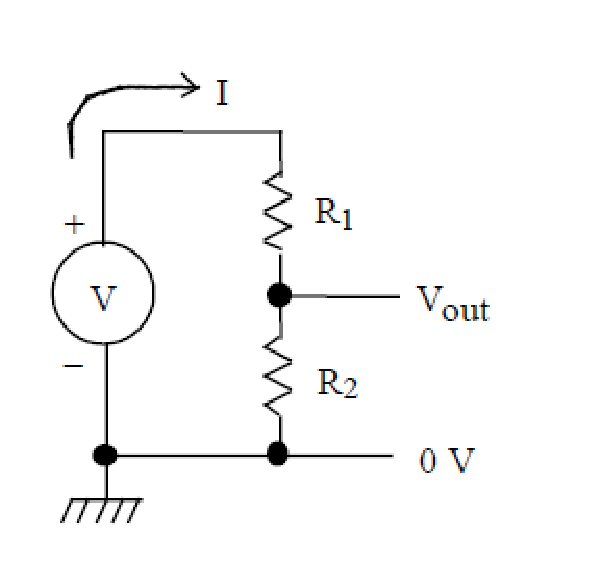
\includegraphics[scale=0.75]{Voltdiv.eps}
\caption{\textit{The schematic for the voltage divider}}
\label{Volt.Div}
\end{center}
\end{figure}
Where we used $R_1$ and $R_2$; $R_3$ and $R_4$; $R_5$ and $R_6$ together to make three different voltage dividers. Then we used the DC power supply to give a $+15\ V$ potential difference from ground into the circuit. Then we measured the voltage out ($V_{out}$) using both the multimeter and the oscilloscope. The values measured are in table \ref{Vout}.
\begin{table}[h]
\begin{center}
\begin{tabular}{ccc|cc}
$R_1$	&$R_2$	&$V_{in}$	&$V_{out}$(Multimeter)	&$V_{out}$(Oscilloscope)\\
\hline
$997\ \Omega$		&$999\ \Omega$		&$15.03\ V$	&$7.50\ V$	&$7.48\ V$\\
$0.997\ M\Omega$	&$0.988\ M\Omega$	&$15.03\ V$	&$7.13\ V$	&$5.00\ V$\\
$9.95\ M\Omega$		&$10.02\ M\Omega$	&$15.03\ V$	&$5.05\ V$	&$1.25\ V$
\end{tabular}
\end{center}
\caption{\textit{The resistances and $V_{in}$ were measured using the digital multimeter. Note that $R_1$ and $R_2$ refer to the resistors in figure \ref{Volt.Div}}}
\label{Vout}
\end{table}
We see that the measured voltages do not agree. We can explain this by realizing that the oscilloscope has a $1.0\ M\Omega$ resistor in parallel with $R_2$ (see figure \ref{Volt.Para}). 
\begin{figure}[h]
\begin{center}
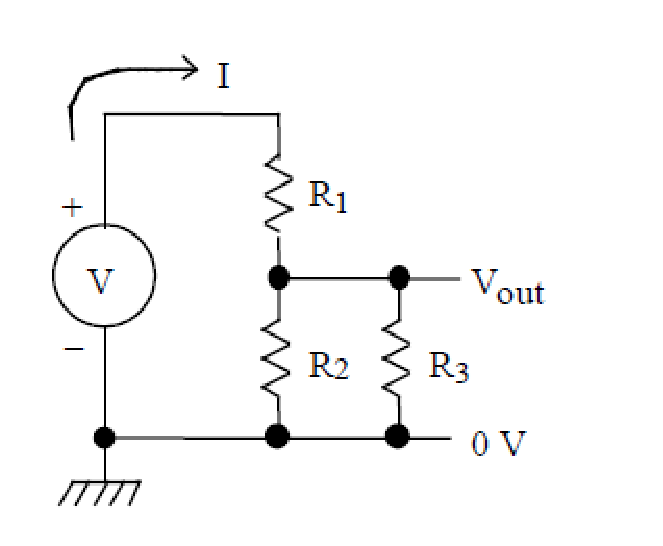
\includegraphics[scale=0.75]{VoltdivPara.eps}
\caption{\textit{The schematic for the voltage divider including the internal resistor of the oscilloscope.}}
\label{Volt.Para}
\end{center}
\end{figure}
We can account for this change by saying the actual resistance in the voltage divider ($R_2$ in figure \ref{Volt.Div}) is the sum of $R_2$ and $R_3$ in parallel using 
\begin{equation}
R_2' = \frac{R_2R_3}{R_2+R_3}
\label{respara}
\end{equation}
where $R_2'$ is the equivalent resistance for $R_2$ in figure \ref{Volt.Div}. Using this fact we calculated the expected value for the voltage out from
\begin{equation}
V_{out} = V_{in}\frac{R_2}{R_1+R_2}
\label{VoltDivEQ}
\end{equation}
(to see the calculated values see table \ref{VoltExp}).
\begin{table}[h]
\begin{center}
\begin{tabular}{cc|ccc}
\multicolumn{2}{c}{Multimeter}	&\multicolumn{3}{c}{Oscilloscope}\\
$V_{out}$(Expected)	&$V_{out}$(Measured) &$R_2'$	&$V_{out}$(Expected)	&$V_{out}$(Measured)\\
\hline
$7.52\ V$	&$7.50\ V$	&$999\ \Omega$		&$7.52\ V$	&$7.48\ V$\\
$7.48\ V$	&$7.13\ V$	&$0.497\ M\Omega$	&$5.00\ V$	&$5.00\ V$\\
$5.03\ V$	&$5.05\ V$	&$0.909\ M\Omega$	&$1.26\ V$	&$1.25\ V$
\end{tabular}
\end{center}
\caption{\textit{A comparison table between the calculated voltage out and the measured voltage out. Note that $R_2'$ was calculated using equation \ref{respara} and both $V_{out}$ values were calculated using \ref{VoltDivEQ}. Also the expected and measured voltage for the $10.0\ M\Omega$ resistors is low because of the $10.0 M\Omega$ internal resistor in the multimeter so $R_2' = 5.01\ M\Omega$ for this circuit.}}
\label{VoltExp}
\end{table}
\subsection{Part \#2}
Using $R_1$ and $R_2$ from table \ref{Meas.Res} and a $10\ k\Omega$ 10-turn potentiometer we built a Wheatstone bridge using figure \ref{Wbridge}. 
\begin{figure}[h]
\begin{center}
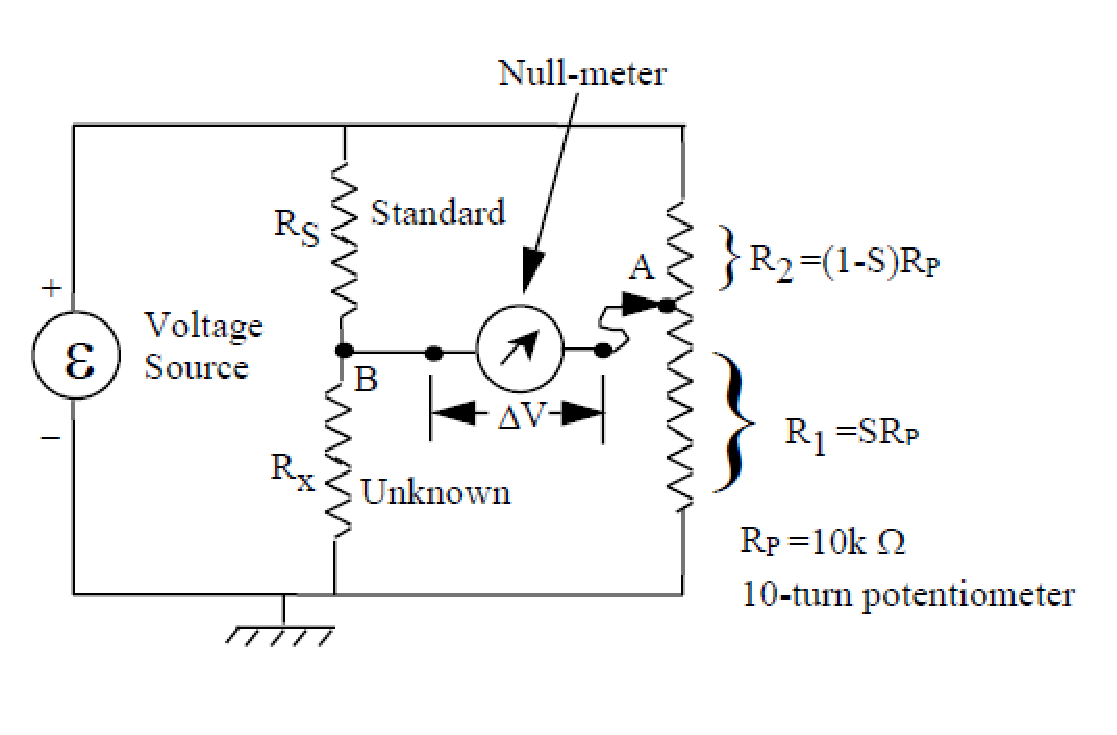
\includegraphics[scale=0.65]{WheatBridge.eps}
\caption{\textit{The schematic for the Wheatstone bridge}}
\label{Wbridge}
\end{center}
\end{figure}
We did this by connecting the two $1.0\ k\Omega$ resistors ($R_s$ and $R_x$) in series then we connected one end of $R_p$ (the full resistor in the potentiometer) and the positive voltage source to $R_s$ (the end not connected to $R_x$). Then we connected the other end of $R_p$ and the ground to $R_x$ (the end not connected to $R_s$). Finally we connected the leads of the multimeter to the connection between $R_s$ and $R_x$ and the resistance divider lead of the potentiometer. Then we turned the voltage on and adjusted the potentiometer until there was no voltage difference. Once we did this we measured the two resistors in the potentiometer (these values are in table \ref{Values}). Next we added a small valued resistor ($\Delta R_x = 15\ \Omega$) in series with $R_x$ and found the change in voltage $\Delta V$
\begin{table}[h]
\begin{center}
\begin{tabular}{c|c}
Component	&Measured Value\\
\hline
$R_s$		&$997\ \Omega$\\
$R_x$		&$999\ \Omega$\\
$R_1$		&$5.09\ k\Omega$\\
$R_2$		&$5.06\ k\Omega$\\
\hline
$\Delta R_x$	&$14.7\ \Omega$\\
$\Delta V$	&$0.056\ V$
\end{tabular}
\caption{\textit{Measured values of the Wheatstone bridge. These were measured with the digital multimeter. Note that $R_1$ and $R_2$ refer to figure \ref{Wbridge}.}}
\label{Values}
\end{center}
\end{table}
We then calculated the expected change in voltage by using the equation
\begin{equation}
\Delta V = \epsilon\left(\frac{\Delta R_x}{R_x}\right)(1-S_0)(S_0) 
\label{deltaV}
\end{equation}
Where $S_0$ is the scale factor of $R_1$ and $R_2$ with $R_p$ given by
$$R_1 = S_0R_p$$ 
and
$$R_2 = (1-S_0)R_p$$ 
So we can calculate $S_0$ by finding the ratio
$$\frac{R_1}{R_1+R_2} = \frac{S_0R_p}{S_0R_p+(1-S_0)R_p}$$
we see that the $R_p$ terms cancel so we get
$$\frac{S_0R_p}{S_0R_p+(1-S_0)R_p} = \frac{S_0}{S_0+1-S_0} = S_0$$
So we can calculate $S_0$ from
\begin{equation}
S_0 = \frac{R_1}{R_1+R_2}
\label{Szero}
\end{equation}
So from equation \ref{Szero} we see that $S_0 = 0.501$. Now we can calculate $\Delta V$ from equation \ref{deltaV}
\begin{align*}
\Delta V &= \epsilon\left(\frac{\Delta R_x}{R_x}\right)(1-S_0)(S_0) \\
&= (15.03)\left(\frac{14.7}{999}\right)(1-0.501)(0.501) \\
&= 0.055\ V
\end{align*}
Note that this is in agreement with the measured result.

\subsection{Part \#3}
For this part we first cut 21 gauge wire to a length $l$ where $l = 72\pm0.2\ in$. We then calculated the diameter of the wire using the fact that the wire is 21 gauge and 
\begin{equation}
\textnormal{AWG gauge} = 30 - 20\log_{10}\left(\frac{d}{0.01"}\right)
\label{gauge}
\end{equation}
using equation \ref{gauge} we found that the diameter of the wire $s$ is $d = 0.028\ in$. Note that now we need to convert inches to centimeters by multiplying by 2.54. This makes the dimensions of the wire $l = 182.9\pm0.05\ cm$ and $d = 0.071\ cm$. We then calculated the cross sectional area by using the formula for the area of a circle
$$A = \pi (d/2)^2$$
and found that $A = 0.0040\ cm^2$. We then stripped the ends cleanly as to get the best connection and used the digital multimeter to find the resistance of the wire. We found the resistance to be $R_{wire} = 0.0\pm0.2\ \Omega$. Now using the relation
$$R = \frac{\rho l}{A}$$
where we solved for the resistivity $\rho$
\begin{equation}
\rho = \frac{R A}{l}
\label{resistanc}
\end{equation}
We calculated $\rho$ by
\begin{align*}
\rho &= \frac{R A}{l}\\
&= \frac{(0)(0.0040)}{182.9}\\
&= 0\ \mu\Omega\ cm
\end{align*}
Now we can find the error in in $\rho$ by saying
\begin{equation}
\Delta\rho = \sqrt{\left(\frac{\partial \rho}{\partial R}\Delta R\right)^2 + \left(\frac{\partial \rho}{\partial l}\Delta l\right)^2}
\label{drho}
\end{equation}
Where $\Delta R$ and $\Delta l$ are the error in $R$ and $l$. So we calculate equation \ref{drho} as
\begin{align*}
\Delta\rho &= \sqrt{\left(\frac{\partial \rho}{\partial R}\Delta R\right)^2 + \left(\frac{\partial \rho}{\partial l}\Delta l\right)^2}\\
&= \sqrt{\left(\frac{A}{l}\Delta R\right)^2 + \left(\frac{R A}{l^2}\Delta l\right)^2}\\
&= \sqrt{\left(\frac{0.0040}{182.9}(0.2)\right)^2 + \left(\frac{(0)(0.0040)}{(182.9)^2}(0.072)\right)^2}\\
&= 0.000004\ \Omega\ cm = 4\ \mu\Omega\ cm
\end{align*}
So our value for $\rho$ is
$$\rho = 0\pm4\ \mu\Omega\ cm$$
We then calculated $R_{wire}$ another way using \emph{Ohm's Law}
\begin{equation}
R = \frac{V}{I}
\label{ohms}
\end{equation}
To do this we measured the current coming out of the power supply and got $I = 1.01\pm0.02 A$ then we connected a voltmeter across the wire and read the potential difference as $V = 0.076\pm0.002\ V$. Then we calculated the resistance from equation \ref{ohms} to get $R_{wire} = 0.075$ we calculated the error on this value as
\begin{align*}
\Delta R &= \sqrt{\left(\frac{\partial R}{\partial V}\Delta V\right)^2+\left(\frac{\partial R}{\partial I}\Delta I\right)^2}\\
&= \sqrt{\left(\frac{1}{I}\Delta V\right)^2+\left(\frac{V}{I^2}\Delta I\right)^2}\\
&= \sqrt{\left(\frac{1}{1.01}(0.002)\right)^2+\left(\frac{0.076}{(1.01)^2}(0.02)\right)^2}\\
&= 0.002\ \Omega
\end{align*}
So the resistance is $R_{wire} = 0.075\pm0.002\ \Omega$. Using equation \ref{resistanc} we find the resistivity of copper as $\rho = 1.64\ \mu\Omega\ cm$. We calculate the error using equation \ref{drho} to get 
\begin{align*}
\Delta\rho &= \sqrt{\left(\frac{\partial \rho}{\partial R}\Delta R\right)^2 + \left(\frac{\partial \rho}{\partial l}\Delta l\right)^2}\\
&= \sqrt{\left(\frac{A}{l}\Delta R\right)^2 + \left(\frac{R A}{l^2}\Delta l\right)^2}\\
&= \sqrt{\left(\frac{0.0040}{182.9}(0.002)\right)^2 + \left(\frac{(0.075)(0.0040)}{(182.9)^2}(0.05)\right)^2}\\
&= 0.04\ \mu\Omega\ cm
\end{align*}
We see that the accuracy of the measurement using \emph{Ohm's Law} is much greater that that of the digital multimeter. This is because the resistance of the wire is such a small value it is very difficult to measure it directly. Through measuring larger quantities such as voltage and current we can calculate the resistance with less error than a direct measurement.
\begin{table}[ht]
\begin{center}
\begin{tabular}{cccc}
		&Expected Value			&\multicolumn{2}{c}{Measured Value}\\
		&						&Direct Multimeter		&Ohm's Law \\
\hline
$\rho$	&$1.68\ \mu\Omega\ cm$	&$0\pm4\ \mu\Omega\ cm$	&$1.64\pm0.04\ \mu\Omega\ cm$
\end{tabular}
\end{center}
\caption{\textit{The measured values of $\rho$ compared to the expected value.}}
\label{rhomeas}
\end{table}
\section{Conclusion}
This experiment demonstrated basic ideas that we be important in future experiments. The usage us the breadboard and the oscilloscope to measure voltage changes. As well as basic circuit construction. We also see that we need to be mindful of the internal resistances in the devices we measure. While we idealize them in theory, in practice no device in ideal and these differences need to be compensated for. 


\end{document}

